% !TeX root = ../main.tex

\section{Deterministic Model}
    \frame{\sectionpage}

    \begin{frame}{Seat Planning with Social Distancing}
      Group type $[M] = \{1, \ldots, M\}$
      Row $[N] = \{1, \ldots, N\}$
      Let $n_i = i + s$ denote the new size of group type $i$ for each $i \in [M]$.
      Let $L_j = S_j + s$ denote the length of row $j$ for each $j \in [N]$, where $S_j$ represents the number of seats in row $j$.
      \begin{figure}[ht]
        \centering
        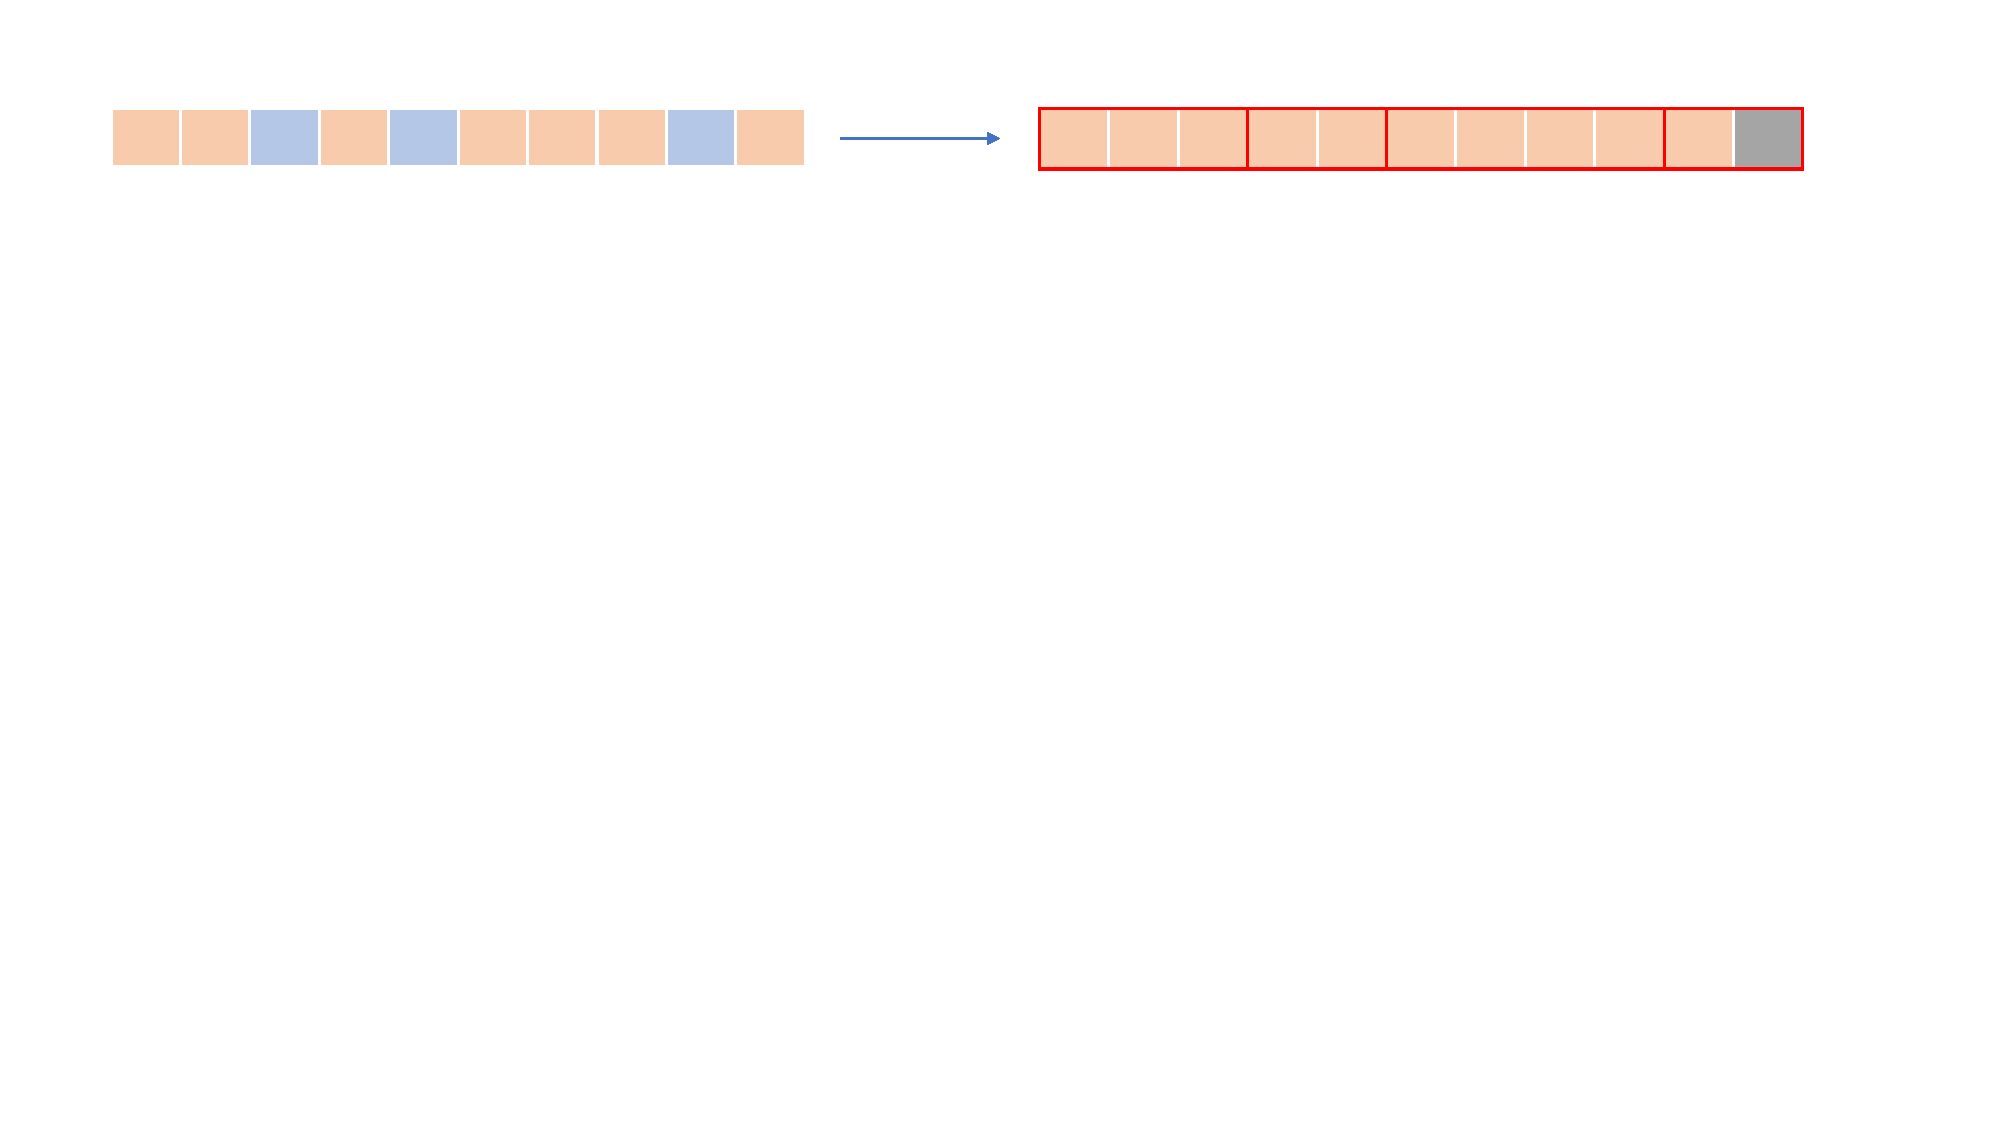
\includegraphics[width = 0.8\textwidth]{./images/dummy_seat.pdf}
        \caption{Problem Conversion}
    \end{figure}

    \end{frame}

    \begin{frame}{Formulation}
      When $|\Omega| =1$ in problem \eqref{sto_form}, the stochastic programming will be 
      \small
      \begin{equation}\label{one_form}
        \begin{aligned}
        \max \quad & \sum_{i=1}^{M}  \sum_{j= 1}^{N} (n_i-s) x_{ij} - \sum_{i=1}^{M} y_{i}^{+}  \\
        \text {s.t.} \quad & \sum_{j= 1}^{N} x_{ij} - y_{i}^{+}+ y_{i+1}^{+} + y_{i}^{-} = d_{i}, \quad i \in [M-1], \\
        & \sum_{j= 1}^{N} x_{ij} -y_{i}^{+} + y_{i}^{-} = d_{i}, \quad i = M, \\
        & \sum_{i=1}^{M} n_{i} x_{ij} \leq L_j, j \in [N]\\
        & y_{i}^{+}, y_{i}^{-} \in \mathbb{Z}_{+}, \quad i \in [M] \\
        & x_{ij} \in \mathbb{Z}_{+}, \quad i \in [M], j \in [N].
        \end{aligned}
      \end{equation}
    \end{frame}

    \begin{frame}{Formulation}
      \begin{equation}\label{deter_upper}
        \begin{aligned}
        \max \quad & \sum_{i=1}^{M}  \sum_{j= 1}^{N} (n_i- s) x_{ij} \\
        \text {s.t.} \quad & \sum_{j= 1}^{N} x_{ij} \leq d_{i}, \quad i \in [M], \\
        & \sum_{i=1}^{M} n_{i} x_{ij} \leq L_j, j \in [N] \\
        & x_{ij} \in \mathbb{Z}_{+}, \quad i \in [M], j \in [N].
        \end{aligned}
      \end{equation}
    \end{frame}

    \begin{frame}{Analysis}

    \end{frame}

    \begin{frame}{Example}
      Suppose the social distancing is one seat, then the new sizes of groups are $2, 3, 4, 5$, respectively. The length of one row is $L = 21$ and the demand is $[10, 12, 9, 8]_d$. Then these patterns, $(5, 5, 5, 5, 1), (5, 4, 4, 4, 4),(5, 5, 5, 3, 3)$, belong to $I_1$. For pattern 1, $(5, 5, 5, 5, 1)$, $P_{1} = \{5\}$, thus a group with a size smaller than 5 cannot be put in this pattern.
    \end{frame}

    \begin{frame}{Properties}
      \begin{itemize}
        \item $\alpha_k$ indicates the number of items for pattern $k$. $\beta_k$ indicates the left space for maximal pattern $k$. Notice that the left space is the true loss.
        \item Denote $\alpha_k + \beta_k- 1$ as the loss for pattern k, $l(k)$. When $l(k)$ reaches minimum, the corresponding pattern $k$ is the optimal solution for a single row.
        \item If the group sizes are consecutive integers starting from 2, $\{2,3,\ldots,u\}$, then a greedy-based pattern is optimal, i.e., select the maximal group size,$u$, as many as possible and the left space is occupied by the group with the corresponding size. The loss is $k+1$, where $k$ is the number of times $u$ selected. Let $S = u\cdot k + r$.
      \end{itemize}
    \end{frame}

    \begin{frame}
      \begin{itemize}
        \item Let $I_1$ be the set of patterns with the minimal loss.
        \item For a seat layout, $\{S_1, S_2, \ldots, S_{N}\}$, the total loss is $\sum_{j} (\lfloor \frac{S_j+1}{u} \rfloor - f((S_j +1)\mod u))$. The maximal number of people assigned is $\sum_{j} (S_j - \lfloor \frac{S_j+1}{u} \rfloor + f((S_j +1)\mod u))$.
      \end{itemize}
    \end{frame}



    % \begin{frame}{Extension}
    %
    % \end{frame}
